

This section demonstrates application of TPG-algebra to designing
processor microcontrollers. Specification of such a complex system
as a processor has to start at the architectural level, which helps
to manage the system complexity by structural abstraction~\cite{1994_de_micheli_book}.

Fig.~\ref{app-fig-Architecture-of-example} shows the architecture
of an example processor. Separate \emph{Program memory} and \emph{Data
memory} blocks are accessed via the \emph{Instruction fetch} (IFU)
and \emph{Memory access} (MAU) units, respectively. The other two
operational units are: \emph{Arithmetic logic unit} (ALU) and \emph{Program
counter increment unit} (PCIU). The units are controlled using request-acknowledgement
interfaces (depicted as bidirectional arrows) by the\textbf{\emph{
}}\emph{Central microcontroller}, which is our primary design objective. 

The processor has four registers: two general purpose registers $A$
and $B$, \emph{Program counter} (PC) storing the address of the current
instruction in the program memory, and the \emph{Instruction register}
(IR) storing the \emph{opcode} (operation code) of the current instruction.
For the purpose of this chapter, the actual width of the registers (the
number of bits they can store) is not important. ALU has access to
all the registers via the register bus; MAU has access to general
purpose registers only; IFU, given the address of the next instruction
in PC, reads its opcode into IR; and PCIU is responsible for incrementing
PC (moving to the next instruction). The microcontroller has access
to the IR and ALU \emph{flags} (information about the current state
of ALU which is used in branching instructions).

Now we define the set of instructions of the processor. Rather than
listing all the instructions, we describe classes of instructions
with the same \emph{addressing mode}~\cite{mspmanual} and the same
execution scenario. As the scenarios here are partial orders of actions,
we use TPG-algebra, and the corresponding TPGs are shown in Fig.~\ref{app-fig-Scenarios-of-8}.

\textbf{ALU operation Rn to Rn}\quad{}An instruction from this class
takes two operands stored in the general purpose registers ($A$ and
$B$), performs an operation, and writes the result back into one
of the registers (so called \emph{register direct addressing mode}).
Examples: $\mathit{ADD\ A,\ B}$ -- addition $A:=A+B$; $\mathit{MOV\ B,\ A}$
-- assignment $B:=A$. ALU works concurrently with PCIU and IFU, which
is captured by the expression $\mathit{ALU}+\mathit{PCIU\rightarrow\mathit{IFU}}$;
the corresponding PG is shown in Fig.~\ref{app-fig-Scenarios-of-8}(a).
As soon as both concurrent branches are completed, the processor is
ready to execute the next instruction. Note that it is not important
for the microcontroller which particular ALU operation is being executed
($\mathit{ADD}$, $\mathit{MOV}$, or any other instruction from this
class) because the scenario is the same from its point of view (it
is the responsibility of ALU to detect which operation it has to perform
according to the current opcode). 


\begin{figure}
\begin{centering}
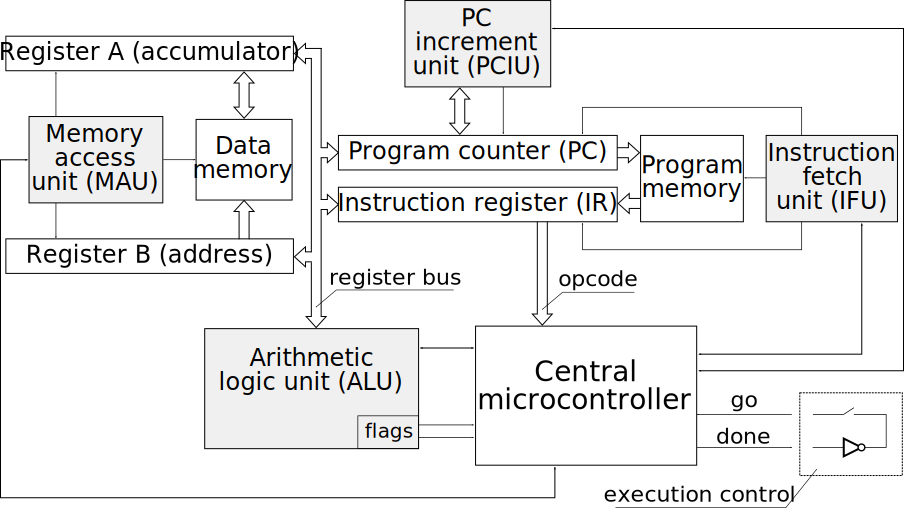
\includegraphics[width=1.04\columnwidth]{fig/processor_architecture}
\par\end{centering}
\caption{Architecture of an example processor\label{app-fig-Architecture-of-example}}
\vspace{-6mm}
\end{figure}


\begin{figure*}
\begin{centering}
\subfloat[ALU op. Rn to Rn]{

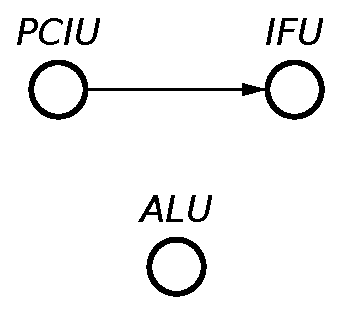
\includegraphics[scale=0.42]{fig/po_ALU_Rn_Rn}}\hfill{}\subfloat[ALU op. \#123 to Rn]{

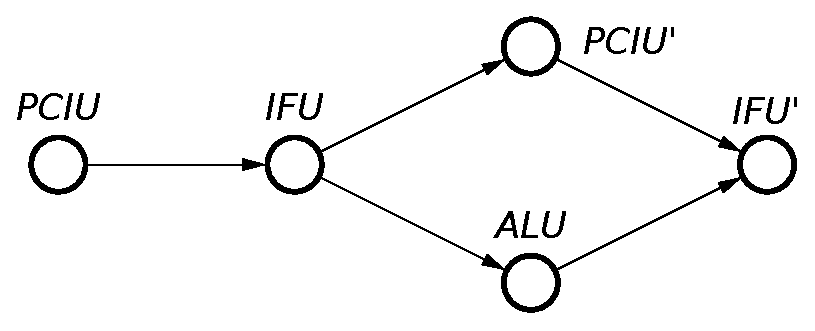
\includegraphics[scale=0.42]{fig/po_ALU_123_Rn}}\hfill{}\subfloat[ALU op. Rn to PC]{


\includegraphics[scale=0.42]{fig/po_ALU_Rn_PC}}\hfill{}\subfloat[ALU op. \#123 to PC]{

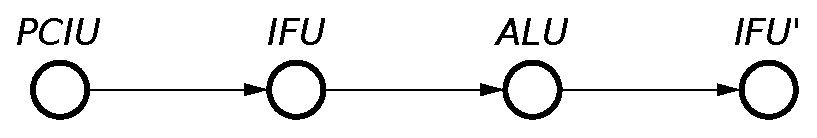
\includegraphics[scale=0.42]{fig/po_ALU_123_PC}}
\par\end{centering}

\begin{centering}
\subfloat[Memory access]{

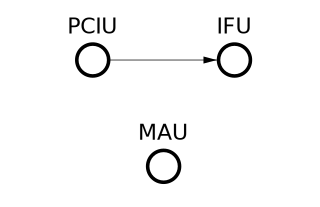
\includegraphics[scale=0.42]{fig/po_MAU}}\hfill{}\subfloat[Cond. ALU op. Rn to Rn]{

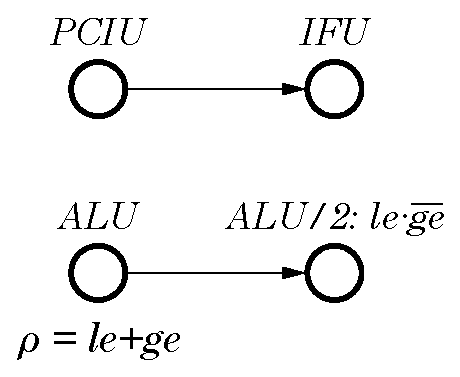
\includegraphics[scale=0.42]{fig/po_CALU_Rn_Rn}}\hfill{}\subfloat[Cond. ALU op. \#123 to Rn]{

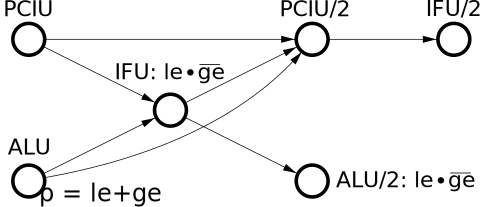
\includegraphics[scale=0.42]{fig/po_CALU_123_Rn}}\hfill{}\subfloat[Cond. ALU op. \#123 to PC]{

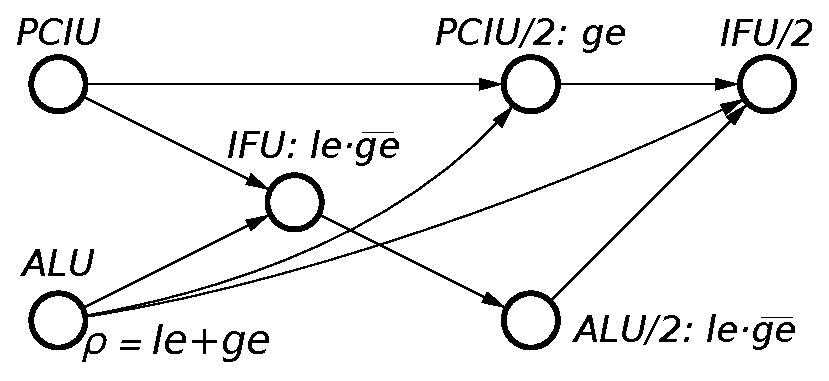
\includegraphics[scale=0.42]{fig/po_CALU_123_PC}}
\par\end{centering}

\caption{TPG specifications of instruction classes\label{app-fig-Scenarios-of-8}}
\vspace{-6mm}
\end{figure*}


\textbf{ALU operation \#123 to Rn}\quad{}In this class of instructions
one of the operands is a register and the other is a constant which
is given immediately after the instruction opcode (e.g. $\mathit{SUB\ A,\ \#5}$
-- subtraction $A:=A-5$), so called \emph{immediate addressing mode}.
At first, the constant has to be fetched into IR, modelled as $\mathit{PCIU}\rightarrow\mathit{IFU}$.
Then ALU is executed concurrently with another increment of PC: $\mathit{ALU}+\mathit{PCIU'}$
(we use $'$ to distinguish the different occurrences of actions of
the same unit). Finally, it is possible to fetch the next instruction
into IR: $\mathit{IFU'}$. The overall scenario is then $\mathit{PCIU}\rightarrow\mathit{IFU}\rightarrow(\mathit{ALU}+\mathit{PCIU'})\rightarrow\mathit{IFU'}$.

\textbf{ALU operation Rn to PC}\quad{}This class contains operations
for unconditional branching, in which PC register is modified. Branching
can be absolute or relative: $\mathit{MOV\ PC,\ A}$ -- absolute branch
to address stored in register $A$, $PC:=A$; $\mathit{ADD\ PC,\ B}$
-- relative branch to the address $B$ instructions ahead of the current
address, $PC:=PC+B$. The scenario is very simple in this case: $\mathit{ALU}\rightarrow\mathit{IFU}$.

\textbf{ALU operation \#123 to PC}\quad{}Instructions in this class
are similar to those above, with the exception that the branch address
or offset is specified explicitly as a constant. The execution scenario
is composed of : $\mathit{PCIU}\rightarrow\mathit{IFU}$ (to fetch
the constant), followed by an ALU operation, and finally by another
IFU operation, $\mathit{IFU'}$. Hence, the overall scenario is $\mathit{PCIU}\rightarrow\mathit{IFU}\rightarrow\mathit{ALU}\rightarrow\mathit{IFU'}$.

\textbf{Memory access}\quad{}There are two instructions in this class:
$\mathit{MOV\ A,\ [B]}$ and $\mathit{MOV\ [B],\ A}$. They load/save
register $A$ from/to memory location with address stored in register
$B$. Due to the presence of separate program and data memory access
blocks, this memory access can be performed concurrently with the
next instruction fetch: $\mathit{PCIU}\rightarrow\mathit{IFU}+\mathit{MAU}$.

\textbf{Conditional instructions}\quad{}These three classes of instructions
are similar to their unconditional versions above with the difference
that they are performed only if the condition $A<B$ holds. The first
ALU action compares registers $A$ and $B$, setting the ALU flag
$lt$ (less than) according to the result of the comparison. This
flag is then checked by the microcontroller in order to decide on
the further scheduling of actions. 

\textbf{Rn~to~Rn}\quad{}This instruction conditionally performs
an ALU operation with the registers (if the condition does not hold,
the instruction has no effect, except changing the ALU flags). The
operation starts with an ALU operation comparing $A$ with $B$; depending
on the result of this comparison, i.e. the status of the flag $lt$,
the second ALU operation may be performed. This is captured by the
expression $\mathit{ALU}\rightarrow[lt]\mathit{ALU'}$. Concurrently
with this, the next instruction is fetched: $\mathit{PCIU}\rightarrow\mathit{IFU}$.
Hence, the overall scenario is $\mathit{PCIU}\rightarrow\mathit{IFU}+\mathit{ALU}\rightarrow[lt]\mathit{ALU'}$.

\textbf{\#123~to~Rn}\quad{}This instruction conditionally performs
an ALU operation with a register and a constant which is given immediately
after the instruction opcode (if the condition does not hold, the
instruction has no effect, except changing the ALU flags). We consider
the two possible scenarios:
\begin{itemize}
\item $A<B$ holds: First, ALU compares $A$ and $B$ concurrently with
a PC increment; since $A<B$ holds, the ALU sets flag $lt$ and the
constant is fetched to the instruction register: $(\mathit{ALU}+\mathit{PCIU})\rightarrow\mathit{IFU}$.
After that PC has to be incremented again, $\mathit{PCIU'}$, and
ALU performs the operation, $\mathit{ALU'}$. Finally, the next instruction
is fetched (it cannot be fetched concurrently with $\mathit{ALU'}$
as ALU is using the constant in IR): $(\mathit{ALU'}+\mathit{PCIU'})\rightarrow\mathit{IFU'}$.
\item $A<B$ does not hold: First, ALU compares $A$ and $B$ concurrently
with a PC increment; since $A<B$ does not hold, the ALU resets flag
$lt$ and the constant that follows the instruction opcode is skipped
by incrementing the PC: $(\mathit{ALU}+\mathit{PCIU})\rightarrow\mathit{PCIU'}$.
Finally, the next instruction is fetched: $\mathit{IFU'}$.
\end{itemize}
\begin{figure*}
\centering
\begin{tabular}{||c||||c||}
\hline 
{\small Instructions class} & {\small Opcode: $xyz$}\tabularnewline
\hline 
\hline 
{\small ALU Rn to Rn} & {\small 000}\tabularnewline
\hline 
{\small ALU \#123 to Rn} & {\small 110}\tabularnewline
\hline 
{\small ALU Rn to PC} & {\small 101}\tabularnewline
\hline 
{\small ALU \#123 to PC} & {\small 010}\tabularnewline
\hline 
{\small Memory access} & {\small 100}\tabularnewline
\hline 
{\small C/ALU Rn to Rn} & {\small 001}\tabularnewline
\hline 
{\small C/ALU \#123 to Rn} & {\small 111}\tabularnewline
\hline 
{\small C/ALU \#123 to PC} & {\small 011}\tabularnewline
\hline 
\end{tabular}

~\\
\vspace{5mm}
~\\

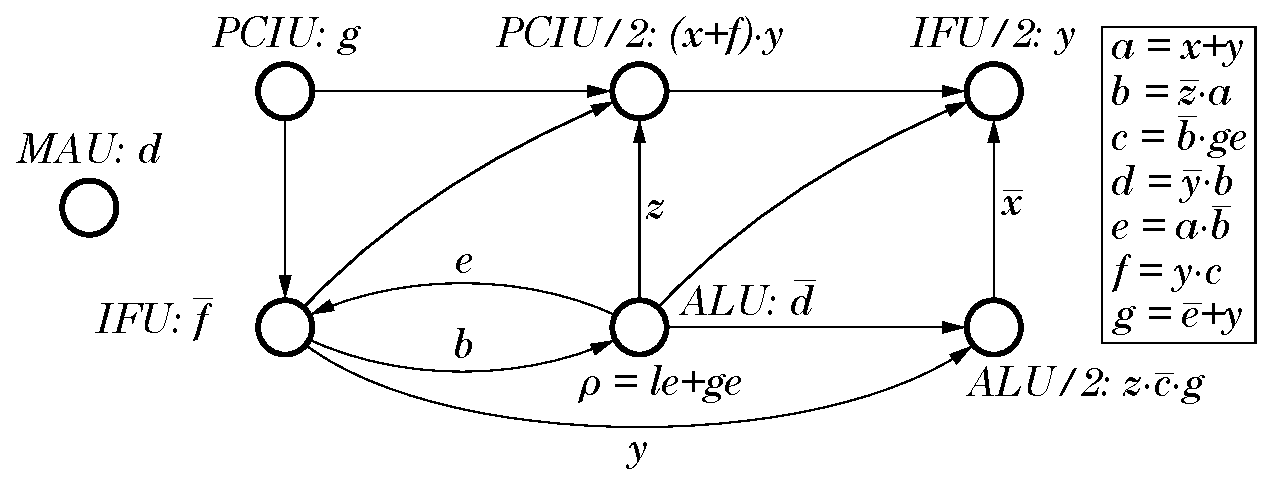
\includegraphics[scale=0.5]{fig/CPOG_L_3}

\caption{Optimal 3-bit instruction opcodes and the corresponding TPG specification
of the microcontroller\label{fig:opcodes-and-CG}}
\vspace{-6mm}
\end{figure*}


Hence, the overall scenario is the overlay of the two subscenarios
above prefixed with appropriate conditions (here we denote the predicate
$A<B$ by $lt$): 
\[
\begin{array}{c}
[lt]((\mathit{ALU}+\mathit{PCIU})\!\rightarrow\!\mathit{IFU}\!\rightarrow\!(\mathit{ALU'}+\mathit{PCIU'})\!\rightarrow\!\mathit{IFU'})+\\
+[\overline{lt}]((\mathit{ALU}+\mathit{PCIU})\!\rightarrow\!\mathit{PCIU'}\!\rightarrow\!\mathit{IFU'}).
\end{array}
\]
This expression can be simplified using the rules of TPG-algebra:%
\footnote{This case illustrates the advantage of using the new hierarchical
approach that allows to specify the system as a composition of scenarios
and formally manipulate them in an algebraic fashion. In our previous work~\cite{cpog_encoding},
the CPOG for this class of instruction
was designed monolithically, and because of this the arc between $\mathit{ALU'}$
and $\mathit{IFU'}$ was missed. Adding this arc not only fixes the
dangerous race between these two blocks, but also leads to a smaller
microcontroller due to the additional similarity between TPGs for
this class of instructions and for the one described below.%
}
\[
(\mathit{ALU}+\mathit{PCIU})\!\rightarrow\![lt]\mathit{IFU}\!\rightarrow\!(\mathit{PCIU'}+[lt]\mathit{ALU'})\!\rightarrow\!\mathit{IFU'}.
\]


\textbf{\#123~to~PC}\quad{}This instruction performs a conditional
branching in which the branch address or offset is specified explicitly
as a constant. We consider the two possible scenarios:
\begin{itemize}
\item $A<B$ holds: First, ALU compares $A$ and $B$ concurrently with
a PC increment; since $A<B$ holds, the ALU sets flag $lt$ and the
constant is fetched to the instruction register: $(\mathit{ALU}+\mathit{PCIU})\rightarrow\mathit{IFU}$.
After that ALU performs the branching operation by modifying PC, $\mathit{ALU'}$.
After PC is changed, the next instruction is fetched, $\mathit{IFU'}$.
\item $A<B$ does not hold: the scenario is exactly the same as in the \textbf{\#123~to~Rn
}case when $A<B$ does not hold.
\end{itemize}
Hence, the overall scenario is the overlay of the two subscenarios
above prefixed with appropriate conditions (here we denote the predicate
$A<B$ by $lt$): 
\[
\begin{array}{c}
[lt]((\mathit{ALU}+\mathit{PCIU})\!\rightarrow\!\mathit{IFU}\!\rightarrow\!\mathit{ALU'}\!\rightarrow\!\mathit{IFU'})+\\
+[\overline{lt}]((\mathit{ALU}+\mathit{PCIU})\!\rightarrow\!\mathit{PCIU'}\!\rightarrow\!\mathit{IFU'}).
\end{array}
\]
This expression can be simplified using the rules of TPG-algebra:
\[
(\mathit{ALU}+\mathit{PCIU})\!\rightarrow\!([\overline{lt}]\mathit{PCIU'}+[lt](\mathit{IFU}\!\rightarrow\!\mathit{ALU'}))\!\rightarrow\!\mathit{IFU'}.
\]


The overall specification of the microcontroller can now be obtained
by prefixing the scenarios with appropriate conditions and overlaying
them. These conditions can be naturally derived from the instruction
opcodes. The opcodes can be either imposed externally or chosen with
the view to optimise the microcontroller. In the latter case, TPG-algebra
and TPGs allow for a formal statement of this optimisation problem
and aid in its solving; in particular, the sizes of the TPG-algebra
expression or TPG are useful measures of microcontroller complexity
(there is a compositional translation from a TPG-algebra expression
into a linear-size circuit). Note that it is natural to use three bits for opcodes as there
are eight classes of instructions, and give an example of optimal
3-bit encoding in the table in Fig.~\ref{fig:opcodes-and-CG}; the
TPG specification of the corresponding microcontroller is shown in
the right part of this figure (the TPG-algebra expression is not shown
because of its size).

